\documentclass[border=4pt]{standalone}
\usepackage{amsmath,amssymb}
\usepackage{tikz}
\usetikzlibrary{arrows.meta,decorations.pathreplacing,patterns,calc,positioning,shapes.geometric}
\usepackage{pgfplots}
\pgfplotsset{compat=newest}
\begin{document}
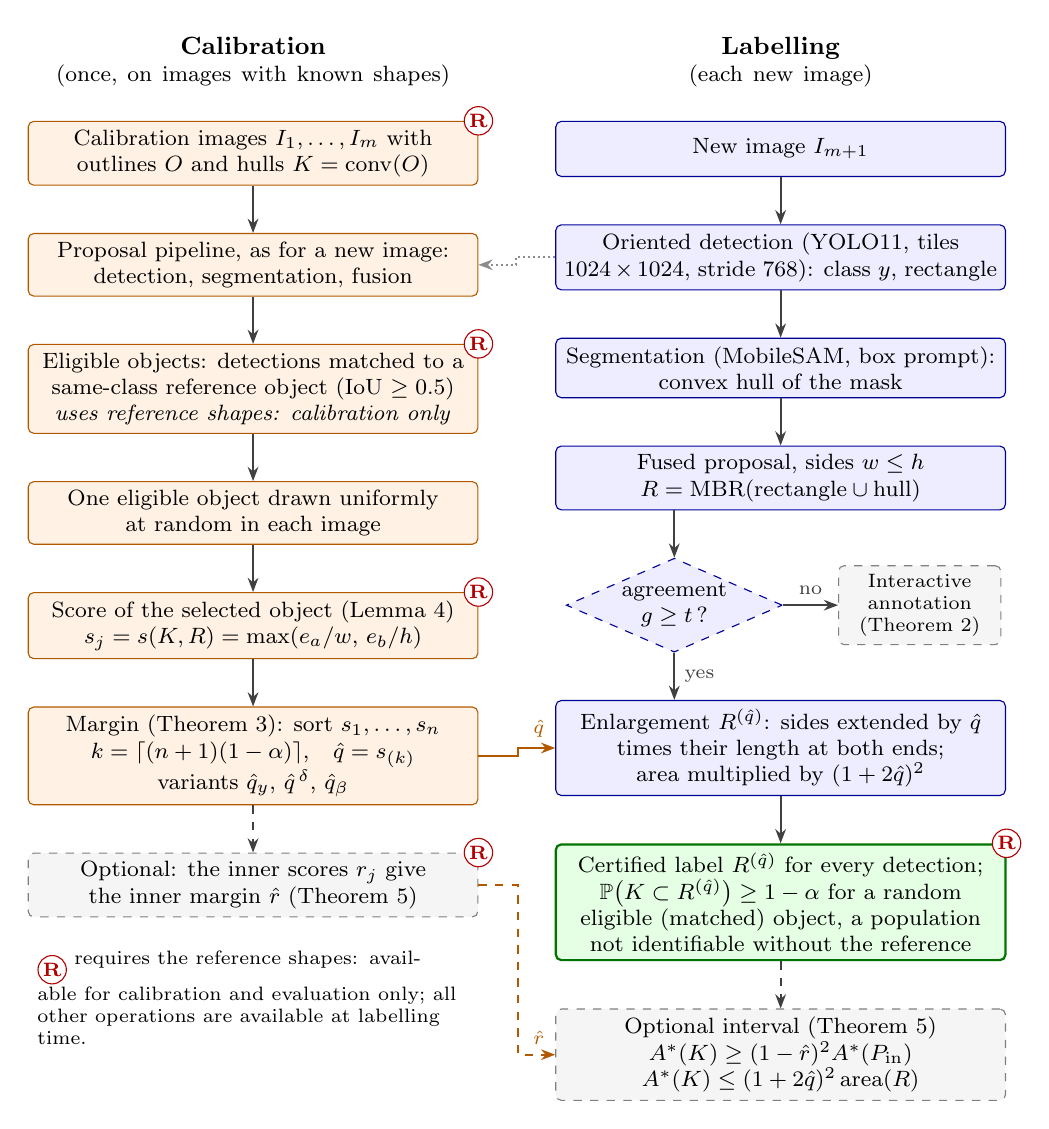
\begin{tikzpicture}[node distance=6mm,
  >={Stealth[length=1.8mm]},
  wbox/.style={draw,rounded corners=2pt,align=flush center,font=\footnotesize,inner sep=3pt,minimum height=7mm},
  wcal/.style={wbox,text width=5.5cm,fill=orange!10,draw=orange!70!black},
  wdep/.style={wbox,text width=5.5cm,fill=blue!7,draw=blue!60!black},
  wout/.style={wbox,text width=5.5cm,fill=green!10,draw=green!45!black,thick},
  wopt/.style={wbox,fill=black!4,draw=black!50,dashed},
  wdec/.style={diamond,dashed,draw=blue!60!black,fill=blue!7,aspect=2.3,font=\footnotesize,inner sep=0.5pt,align=center},
  warr/.style={->,thick,black!75},
  whdr/.style={font=\small\bfseries,align=center,text width=5.4cm},
  wref/.style={circle,draw=red!70!black,fill=white,text=red!70!black,font=\scriptsize\bfseries,inner sep=0.6pt,minimum size=3.6mm}]
\node[whdr,anchor=north] (hc) at (-3.35,0) {Calibration\\[-1pt]{\footnotesize\normalfont(once, on images with known shapes)}};
\node[wcal,below=3mm of hc] (c1) {Calibration images $I_1,\ldots,I_m$ with\\ outlines $O$ and hulls $K=\operatorname{conv}(O)$};
\node[wcal,below=of c1] (c2) {Proposal pipeline, as for a new image:\\ detection, segmentation, fusion};
\node[wcal,below=of c2] (c3) {Eligible objects: detections matched to a\\ same-class reference object (IoU $\ge0.5$)\\ \textit{uses reference shapes: calibration only}};
\node[wcal,below=of c3] (c4) {One eligible object drawn uniformly\\ at random in each image};
\node[wcal,below=of c4] (c5) {Score of the selected object (Lemma~4)\\ $s_j=s(K,R)=\max(e_a/w,\,e_b/h)$};
\node[wcal,below=of c5] (c6) {Margin (Theorem~3): sort $s_1,\ldots,s_n$\\ $k=\lceil(n+1)(1-\alpha)\rceil$,\quad $\hat q=s_{(k)}$\\ variants $\hat q_y$, $\hat q^{\,\delta}$, $\hat q_\beta$};
\node[wopt,text width=5.5cm,below=of c6] (c7) {Optional: the inner scores $r_j$ give\\ the inner margin $\hat r$ (Theorem~5)};
\foreach \a/\b in {c1/c2,c2/c3,c3/c4,c4/c5,c5/c6} \draw[warr] (\a) -- (\b);
\draw[warr,dashed] (c6) -- (c7);
\foreach \n in {c1,c3,c5,c7} \node[wref] at (\n.north east) {R};
\node[font=\scriptsize,align=left,text width=5.4cm,anchor=north west] at ([yshift=-3mm]c7.south west) {\tikz[baseline=-0.6ex]\node[wref]{R};\ requires the reference shapes: available for calibration and evaluation only; all other operations are available at labelling time.};
\node[whdr,anchor=north] (hd) at (3.35,0) {Labelling\\[-1pt]{\footnotesize\normalfont(each new image)}};
\node[wdep,below=3mm of hd] (d1) {New image $I_{m+1}$};
\node[wdep,below=of d1] (d2) {Oriented detection (YOLO11, tiles\\ $1024\times1024$, stride 768): class $y$, rectangle};
\node[wdep,below=of d2] (d3) {Segmentation (MobileSAM, box prompt):\\ convex hull of the mask};
\node[wdep,below=of d3] (d4) {Fused proposal, sides $w\le h$\\ $R=\mathrm{MBR}(\text{rectangle}\cup\text{hull})$};
\node[wdec,below=6mm of d4,xshift=-1.35cm] (d5) {agreement\\ $g\ge t$\,?};
\node[wopt,text width=1.85cm,font=\scriptsize,right=7mm of d5] (m5) {Interactive annotation (Theorem~2)};
\node[wdep,below=6mm of d5,xshift=1.35cm] (d6) {Enlargement $R^{(\hat q)}$: sides extended by $\hat q$\\ times their length at both ends;\\ area multiplied by $(1+2\hat q)^2$};
\node[wout,below=of d6] (d7) {Certified label $R^{(\hat q)}$ for every detection;\\ $\mathbb{P}\big(K\subset R^{(\hat q)}\big)\ge1-\alpha$ for a random\\ eligible (matched) object, a population\\ not identifiable without the reference};
\node[wopt,text width=5.5cm,below=of d7] (d8) {Optional interval (Theorem~5)\\ $A^*(K)\ge(1-\hat r)^2A^*(P_{\mathrm{in}})$\\ $A^*(K)\le(1+2\hat q)^2\,\mathrm{area}(R)$};
\foreach \a/\b in {d1/d2,d2/d3,d3/d4} \draw[warr] (\a) -- (\b);
\draw[warr] (d4.south -| d5.north) -- (d5.north);
\draw[warr] (d5.east) -- node[font=\scriptsize,above]{no} (m5.west);
\draw[warr] (d5.south) -- node[font=\scriptsize,right]{yes} (d5.south |- d6.north);
\draw[warr] (d6) -- (d7);
\draw[warr,dashed] (d7) -- (d8);
\node[wref] at (d7.north east) {R};
\draw[warr,orange!70!black] (c6.east) -- ++(0.5,0) |- node[pos=0.78,above,font=\scriptsize]{$\hat q$} (d6.west);
\draw[warr,orange!70!black,dashed] (c7.east) -- ++(0.5,0) |- node[pos=0.78,above,font=\scriptsize]{$\hat r$} (d8.west);
\draw[warr,black!45,densely dotted] (d2.west) -- ++(-0.5,0) |- (c2.east);
\end{tikzpicture}
\end{document}
